%% Version 4.3.2, 25 August 2014
%
%%%%%%%%%%%%%%%%%%%%%%%%%%%%%%%%%%%%%%%%%%%%%%%%%%%%%%%%%%%%%%%%%%%%%%
% Template.tex --  LaTeX-based template for submissions to the 
% American Meteorological Society
%
% Template developed by Amy Hendrickson, 2013, TeXnology Inc., 
% amyh@texnology.com, http://www.texnology.com
% following earlier work by Brian Papa, American Meteorological Society
%
% Email questions to latex@ametsoc.org.
%
%%%%%%%%%%%%%%%%%%%%%%%%%%%%%%%%%%%%%%%%%%%%%%%%%%%%%%%%%%%%%%%%%%%%%
% PREAMBLE
%%%%%%%%%%%%%%%%%%%%%%%%%%%%%%%%%%%%%%%%%%%%%%%%%%%%%%%%%%%%%%%%%%%%%

%% Start with one of the following:
% DOUBLE-SPACED VERSION FOR SUBMISSION TO THE AMS
%\documentclass{ametsoc}

% TWO-COLUMN JOURNAL PAGE LAYOUT---FOR AUTHOR USE ONLY
 \documentclass[twocol]{ametsoc}

%%%%%%%%%%%%%%%%%%%%%%%%%%%%%%%%
%%% To be entered only if twocol option is used

\journal{mwr}

%  Please choose a journal abbreviation to use above from the following list:
% 
%   jamc     (Journal of Applied Meteorology and Climatology)
%   jtech     (Journal of Atmospheric and Oceanic Technology)
%   jhm      (Journal of Hydrometeorology)
%   jpo     (Journal of Physical Oceanography)
%   jas      (Journal of Atmospheric Sciences)	
%   jcli      (Journal of Climate)
%   mwr      (Monthly Weather Review)
%   wcas      (Weather, Climate, and Society)
%   waf       (Weather and Forecasting)
%   bams (Bulletin of the American Meteorological Society)
%   ei    (Earth Interactions)

%%%%%%%%%%%%%%%%%%%%%%%%%%%%%%%%
%Citations should be of the form ``author year''  not ``author, year''
\bibpunct{(}{)}{;}{a}{}{,}

%%%%%%%%%%%%%%%%%%%%%%%%%%%%%%%%

%%% To be entered by author:

%% May use \\ to break lines in title:

\title{Physics-dynamics coupling with element-based high-order Galerkin methods: quasi equal-area physics grid}

%%% Enter authors' names, as you see in this example:
%%% Use \correspondingauthor{} and \thanks{Current Affiliation:...}
%%% immediately following the appropriate author.
%%%
%%% Note that the \correspondingauthor{} command is NECESSARY.
%%% The \thanks{} commands are OPTIONAL.

    %\authors{Author One\correspondingauthor{Author One, 
    % American Meteorological Society, 
    % 45 Beacon St., Boston, MA 02108.}
% and Author Two\thanks{Current affiliation: American Meteorological Society, 
    % 45 Beacon St., Boston, MA 02108.}}

\authors{Adam R. Herrington\correspondingauthor{Peter H. Lauritzen, Climate and Global Dynamics, National Center for Atmospheric Research, 1850 Table Mesa Drive, Boulder, Colorado, USA.}}

%% Follow this form:
    % \affiliation{American Meteorological Society, 
    % Boston, Massachusetts.}

\affiliation{School of Marine and Atmospheric Sciences, Stony Brook University, State University of New York, Stony Brook, New York.}

%% Follow this form:
    %\email{latex@ametsoc.org}

\email{pel@ucar.edu}

%% If appropriate, add additional authors, different affiliations:
\extraauthor{Peter H. Lauritzen}
\extraaffil{Climate and Global Dynamics, National Center for Atmospheric Research, 1850 Table Mesa Drive, Boulder, Colorado, USA.}
\extraauthor{Steve Goldhaber}
\extraaffil{Climate and Global Dynamics, National Center for Atmospheric Research, 1850 Table Mesa Drive, Boulder, Colorado, USA.}
\extraauthor{Kevin A. Reed}
\extraaffil{School of Marine and Atmospheric Sciences, Stony Brook University, State University of New York, Stony Brook, New York.}

%% May repeat for a additional authors/affiliations:

%\extraauthor{}
%\extraaffil{}

%%%%%%%%%%%%%%%%%%%%%%%%%%%%%%%%%%%%%%%%%%%%%%%%%%%%%%%%%%%%%%%%%%%%%
% ABSTRACT
%
% Enter your abstract here
% Abstracts should not exceed 250 words in length!
%
% For BAMS authors only: If your article requires a Capsule Summary, please place the capsule text at the end of your abstract
% and identify it as the capsule. Example: This is the end of the abstract. (Capsule Summary) This is the capsule summary. 

\abstract{Enter the text of your abstract here.}

\begin{document}

%% Necessary!
\maketitle


%%%%%%%%%%%%%%%%%%%%%%%%%%%%%%%%%%%%%%%%%%%%%%%%%%%%%%%%%%%%%%%%%%%%%
% MAIN BODY OF PAPER
%%%%%%%%%%%%%%%%%%%%%%%%%%%%%%%%%%%%%%%%%%%%%%%%%%%%%%%%%%%%%%%%%%%%%
%

%% In all cases, if there is only one entry of this type within
%% the higher level heading, use the star form: 
%%
\begin{itemize}
\item We should compute TKE of tendencies and show that we ar removing scales with nc<2
\end{itemize}
\section{Introduction}

%this should be included in the next paper (physres)
%When introducing a physics grid separate from the dynamics grid the question arises of what the resolution of the physics grid should be compared to the dynamics grid. For example, Figure \ref{fig:physgrid-1d} shows physics grids with the same, coarser and finer resolution than the GLL dynamics grid. From linear stability and accuracy analysis of numerical methods, it is a common result that the shortest resolvable wavelengths are not accurately represented. Similar arguments can be made from analyzing total kinetic energy spectra \citep{S2011LNCSE}. One may therefore argue that only believable scales should be passed to the physical parameterizations \citep{LH1997MWR}, i.e. a coarser resolution physics grid. This concept was investigated in a spectral transform model by \cite{W1999T}. On the other hand, computing physics tendencies on a higher-resolution grid compared to the dynamical core may provide a better sampling of the atmospheric state, somewhat similar to the super-parameterization \citep{G2001JAS,GRL:GRL14999,SA2007ASL} and sub-columns{\footnote{\citet{gmdd-8-5041-2015} in the context of CAM}} \citep{subcolumn,JGRD:JGRD10481} concepts. This approach was taken by \cite{M2009T} in the context of vertical refinement. \cite{W2014PTRSL} found improved forecast scores by increasing the grid-point space resolution compared to the resolution in wave-number space for the spectral transform model at ECMWF. 

%Alternatively, one could combine the two ideas and compute the state of the atmosphere on a coarser resolution grid and then use sub-columns or super-parameterization. One thereby passes believable scales to the sub-grid scale model and thereby assumes that a statistical sampling, in the case of sub-columns, or a simplified cloud-resolving model, in the case of super-parameterization, provides a more accurate sub-grid-scale tendency than sampling the Galerkin basis functions over the sub-grid-scale. [Discuss \cite{W2014PTRSL}: spectral truncation and physics (physical) grid (see page 10; conclusions)]




%Separating physics and dynamics grids has been investigated in the context of spectral transform models by \citet{TELA:TELA0009}, in which the separation was performed by truncation in wavenumber space. Parts of the physical parameterizations (microphysics) were separated in \citet{JGRD:JGRD50711} and vertical grid separation was investigated in \citet{TELA:TELA394}. In this study we run all of the parameterization on the physgrid.


%In the context of spectral transform model \citet{TELA:TELA0009} held the physics forcing scale fixed while refining the horizontal resolution of the dynamical core. In the context of microphysics \citet{JGRD:JGRD50711} did a scale separation and \citet{TELA:TELA394} separated the vertical grids. While \citet{LH1997MWR} and \citet{TELA:TELA0009} separated scales truncation of the the wave transform, we here separate scales through integrating basis functions over control volumes and , contrary to \citet{JGRD:JGRD50711}, all of the physical parameterization computations are performed on the physgrid. We focus on horizontal separation of scales here.


% \subsection*{subsection}
% text...
\section{Methods}
Separating dynamics, tracer and physics grids introduces the added complexity of having to map the state from dynamics and tracer grids to the physics grid; and mapping physics tracer increments back to the tracer grid and physics increments needed by the dynamical core to the dynamics grid (see Figure \ref{fig:overview}). The dynamics grid in the case of CAM-SE-CSLAM refers to the Gauss-Lobatto-Legendre (GLL) quadrature nodes used by the spectral-element method to solve the momentum equations for the momentum vector $(u,v)$, thermodynamics equation for temperature ($T$), continuity equation for dry air mass ($\frac{1}{g}p$), and continuity equations for water vapor and thermodynamically and inertially active condensates \citep[see, e.g., ][ for details]{LetAl2018JAMES}. By tracer grid we refer to the $pg3$ grid on which CSLAM performs tracer transport of water vapor, condensates and other tracers. Although water vapor and condensates are being advected by the CSLAM scheme on the $pg3$ grid, these quantities are also needed on the GLL grid for the momentum equations and thermodynamic equation. Transport of water variables is also performed by the spectral-element method on the GLL grid. To avoid decoupling of water species on the CSLAM and GLL grids, the GLL water species are overwritten by the CSLAM values every physics time-step. This is explained in detail in H18.

\begin{figure}[t]
\begin{center}
\noindent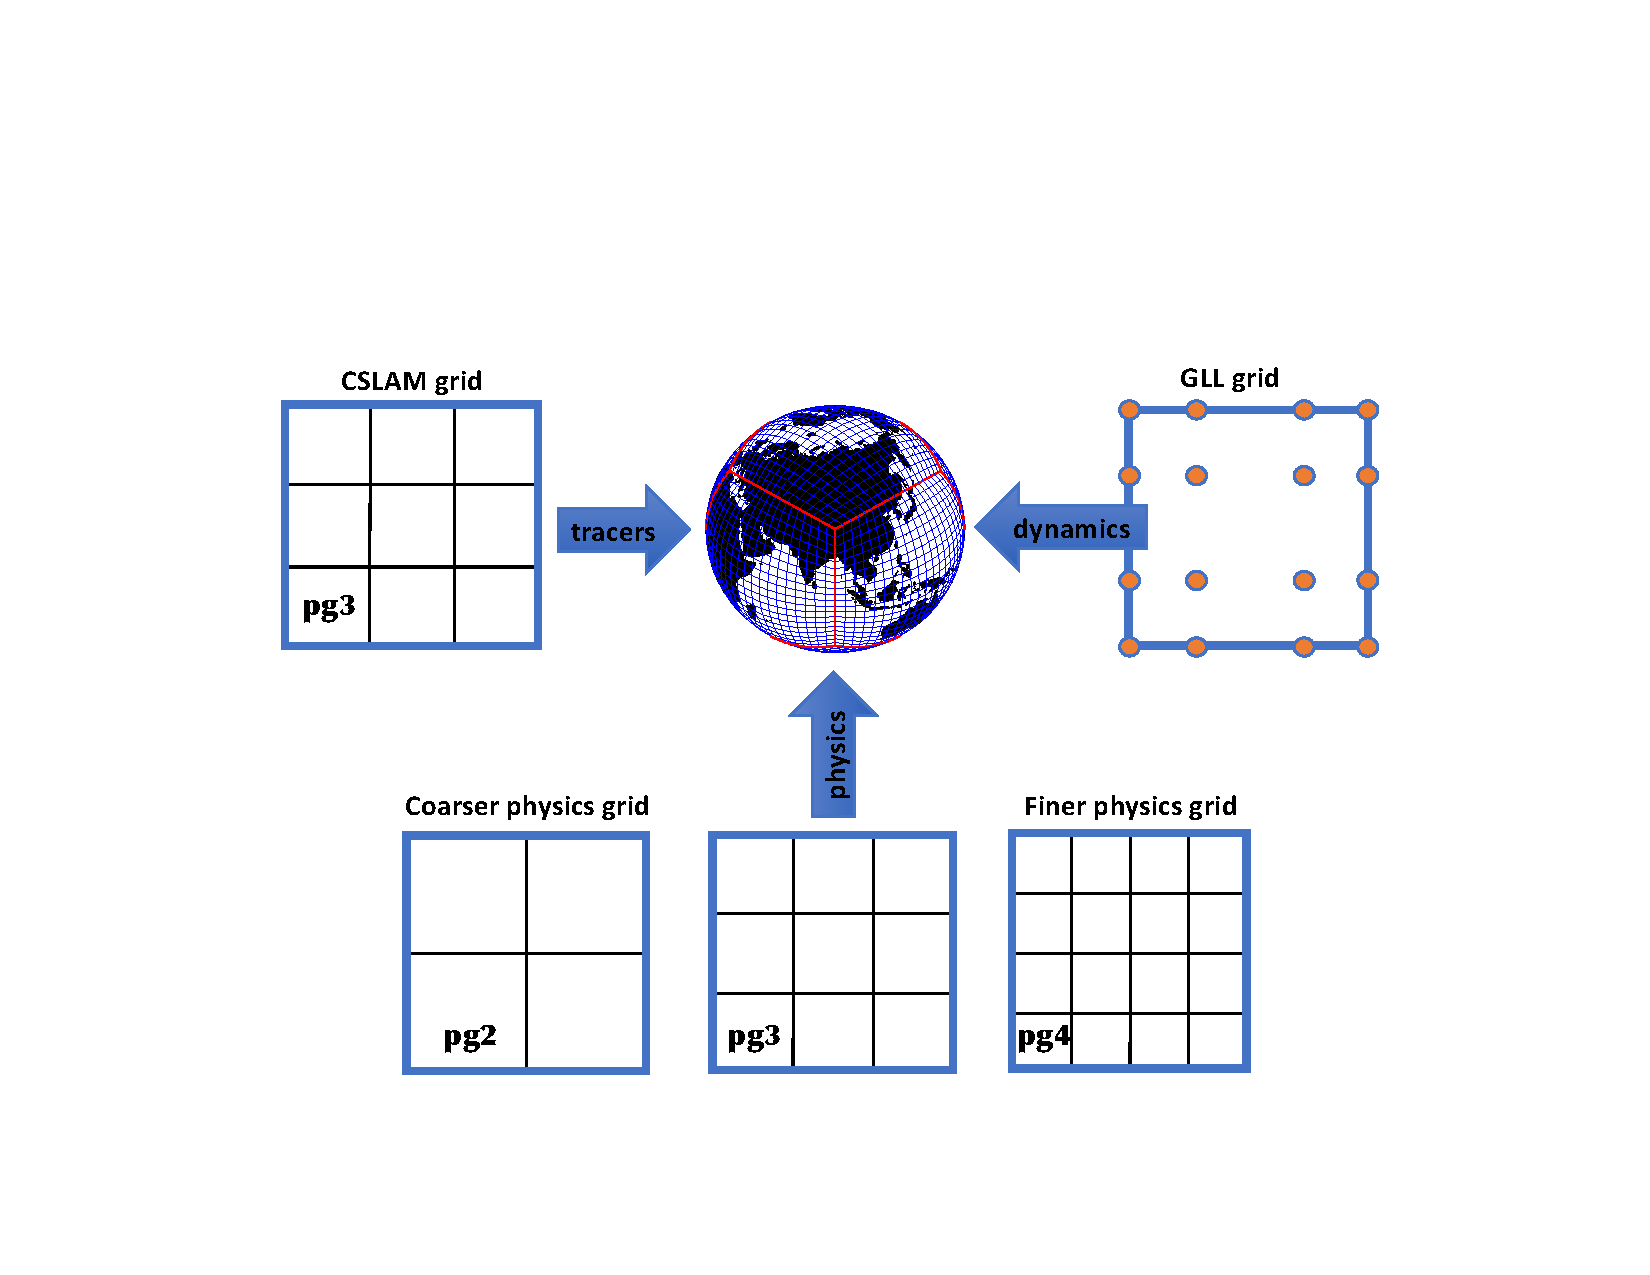
\includegraphics[width=30pc,angle=0]{figs/fig-overview.pdf}\\
\end{center}
\caption{An overview of the different grids in CAM-SE-CSLAM.}
\label{fig:overview}
\end{figure}

Similarly to the CAM-SE-CSLAM $pg3$ configuration, the dynamics state (momentum vector, temperature, dry pressure) must be mapped from the $GLL$ grid to the physics grid. Exactly the same algorithms as used in the $pg3$ configuration apply, i.e. momentum components are interpolated by evaluating the internal Lagrange basis functions (used in the spectral-element method) at the equi-angular (gnomonic) center of the $pg2$ cells and the Lagrange basis function representations of temperature and pressure are integrated over the $pg2$ control volumes. See H18 for details.

As compared to the $pg3$ configuration, the extra complication with the $pg2$ setup is that the tracer grid does not coincide with the physics grid, i.e. the tracer state needs to be mapped from the CSLAM grid ($pg3$) to the physics grid ($pg2$), and tracer increments computed by physics must be mapped from the physics grid back to the CSLAM grid. In order to describe the mapping algorithms between the grids some notation needs to be introduced.

The mapping algorithms are applied to each element $\Omega$ (with spherical area $\Delta \Omega$) so without loss of generality consider one element. Let $\Delta A^{(pg2)}_k$ and $\Delta A^{(pg3)}_\ell$ be the spherical area of the physics grid cell $A^{(pg2)}_k$ and CSLAM control volume $A^{(pg3)}_\ell$, respectively. The physics grid cells and CSLAM cells, respectively, span the element, $\Omega$, without gaps or overlaps
\begin{eqnarray}
\cup_{k=1}^{nphys^2}A^{(pg2)}_k=\Omega \text{ and } A^{(pg2)}_k \cap A^{(pg2)}_\ell = \emptyset \quad \forall k\ne \ell,\\
\cup_{k=1}^{nc^2}A^{(pg3)}_k=\Omega \text{ and } A^{(pg3)}_k \cap A^{(pg3)}_\ell = \emptyset \quad \forall k\ne \ell,
\end{eqnarray}
where $nc=3$ is the CSLAM grid resolution parameter and $nphys=2$ is the physics grid resolution parameter (following the Fortran code base), although the methods described here are valid for any arbitrary integer $nphys$ (e.g., $nphys=4$ is shown in Figure~\ref{fig:overview}). The overlap areas between the $k$-th physics grid cell and $\ell$th CSLAM cell are denoted
\begin{equation}
A_{k\ell}=A^{(pg2)}_k \cap A^{(pg3)}_\ell,
\end{equation}
(see Figure \ref{fig:area-schematic}) so that
\begin{equation}
A^{(pg2)}_k=\cup_{l=1}^{nc^2}A_{k\ell}.
\end{equation}
This overlap grid is also referred to as the {\em{exchange grid}}.
\subsection{Mapping tracers from $A^{(pg3)}$ to $A^{(pg2)}$ (CSLAM to physics grid)}\label{sec:nctopg}
The CSLAM and physics grids are both finite-volume grids so existing CSLAM technology can be used to map the tracer state from CSLAM to physics grid. That is, compute a high-order shape-preserving reconstruction of mixing ratio $m$ and dry air mass  $\frac{1}{g}\Delta p$ per unit area in each CSLAM control volume and integrate those reconstruction functions over the overlap areas \citep{LNU2010JCP,NL2010JCP}. This algorithm retains the properties of CSLAM: inherent mass-conservation, consistency (constant mixing ratio is preserved), mixing ratio shape-preservation and linear-correlation preservation.

\begin{figure}[t]
\begin{center}
\noindent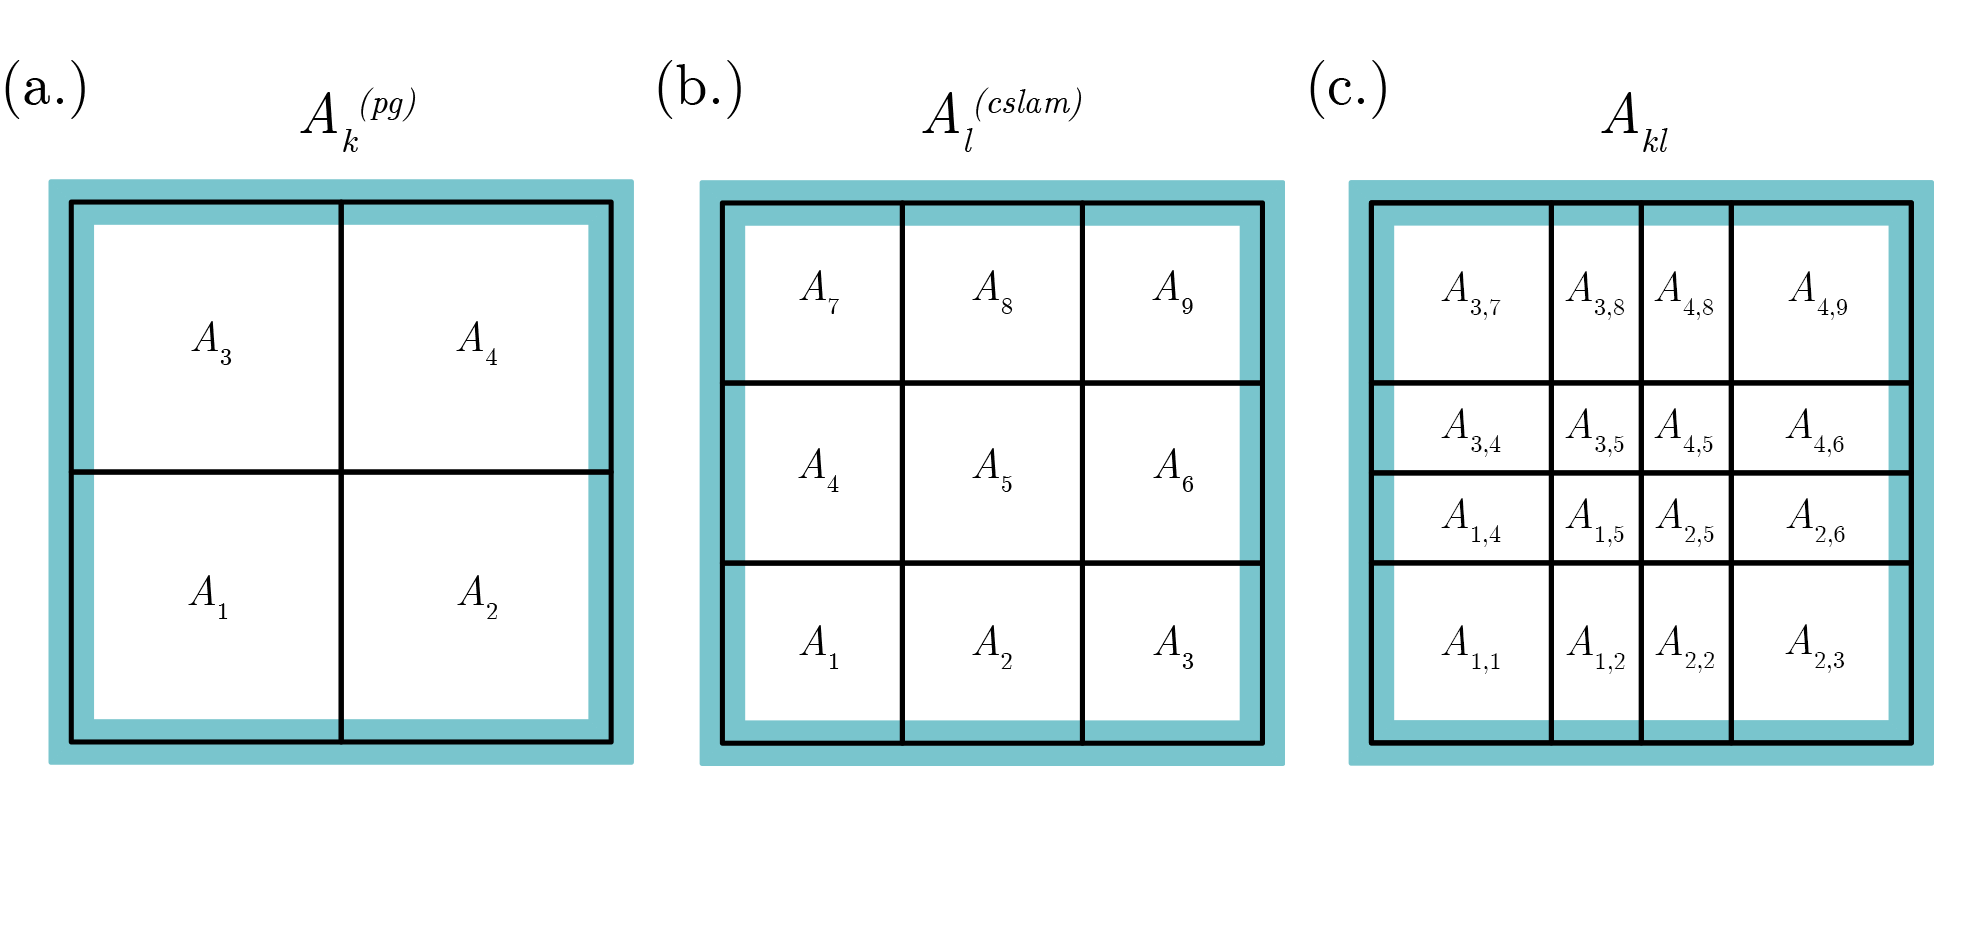
\includegraphics[width=30pc,angle=0]{figs/area-schematic.png}\\
\end{center}
\caption{Indices notation for (a) the $pg2$ grid, (b) the $pg3$ grid and (c) their exchange grid.}
\label{fig:area-schematic}
\end{figure}

Denote the known cell averaged values of dry pressure-level thickness and mixing ratio $\overline{\Delta p}^{(pg3)}$ and $\overline{m}^{(pg3)}$, respectively. We consider a particular layer and for simplicity drop the layer subscript. The same procedure is applied to each layer in a column. The unknowns we would like to compute is the cell-averaged values of the same quantities on the physics grid; $\overline{\Delta p}^{(pg2)}$ and $\overline{m}^{(pg2)}$, respectively. The dry pressure level thickness integrated over the $k$'th physics grid cell is given by
\begin{equation}
\label{eq:p}
\overline{\Delta p}^{(pg2)}_k=\frac{1}{\Delta A^{(pg2)}_k}\sum_{\ell=1}^{nc^2}\left<\delta p\right>_{k\ell},
\end{equation}
where $\left< \delta p\right>_{k\ell}$ is the dry mass in a layer over overlap area $A_{k\ell}$. It is computed by integrating a high-order (2D polynomial of degree 2) reconstruction of pressure-level thickness in each CSLAM cell over the overlap area $A_{k\ell}$
\begin{equation}
\label{eq:pg3dp}
\left< \delta p\right>_{k\ell}=\int_{A_{k\ell}}\left[ \sum_{i+j\le 2}{\mathcal{P}}^{(ij)}_\ell x^{i}y^{j}\right] dA.
\end{equation}
The reconstruction coefficients ${\mathcal{P}}^{(ij)}_\ell$ in CSLAM cell $\ell$ are computed from the cell average pressure level thicknesses on the CSLAM grid $\overline{\Delta p}^{(pg3)}$ and the numerical integration over overlap areas is done by line-integrals. The details of that is given in \cite{LNU2010JCP} and not repeated here.

The average tracer mass per unit area on the physics grid is given by
\begin{equation}
\label{eq:mp}
\overline{m\Delta p}^{(pg2)}_k=\frac{1}{\Delta A^{(pg2)}_k}\sum_{\ell=1}^{nc^2}\left< m\delta p\right>_{k\ell},
\end{equation}
where $\left< m\delta p\right>_{k\ell}$ is the tracer mass over $A_{k\ell}$ resulting from integrating a high-order reconstruction of $\Delta p$ and $m$ combined using the approach outlined in Appendix B of \cite{NL2010JCP} over the overlap area $A_{k\ell}$
\begin{equation}
\label{eq:mp2}
\left< m\delta p\right>_{k\ell}=\int_{A_{k\ell}}\left[ \overline{\Delta p}_\ell^{(pg3)}\sum_{i+j\le 2}{\mathcal{M}}^{(ij)}_\ell x^{i}y^{j}+{\overline{m}}_\ell^{(pg3)}\sum_{i+j\le 2}{\widetilde{{\mathcal{P}}}}^{(ij)}_\ell x^{i}y^{j}\right] dA,
\end{equation}
where ${\widetilde{{\mathcal{P}}}}^{(00)}_\ell={\mathcal{P}}^{(00)}_\ell-\overline{\Delta p}^{(pg3)}_\ell$ and ${\widetilde{{\mathcal{P}}}}^{(ij)}_\ell={\mathcal{P}}^{(ij)}_\ell$ for $i,j>0$, and ${\mathcal{M}}^{(ij)}_\ell$ are the reconstruction coefficients for the mixing ratio in CSLAM cell $A^{(pg3)}_\ell$. A shape-preserving limiter is applied to the reconstruction of mixing ratio $m$ \citep{BJ1989} and not $\Delta p$. This way of combining the reconstruction function for $\Delta p$ and $m$ in \eqref{eq:mp2} ensures that a constant mixing ratio is preserved (consistency), tracer mass is conserved, linear-correlations are preserved and tracer shape-preservation is retained. The mixing ratio on the physics grid is then
\begin{equation}
{\overline{m}}^{(pg2)}_k=\frac{\overline{\left( m\Delta p\right)}^{(pg2)}_k}{\overline{\Delta p}^{(pg2)}_k},
\end{equation}
where $\overline{\Delta p}^{(pg2)}_k$ is given in \eqref{eq:p}. 

Perhaps surprisingly a much more challenging problem is to map tracer increments (or state) from the physics grid to the CSLAM grid while retaining important properties such as mass-conservation, consistency, and correlation preservation. Why this mapping problem is challenging is explained in detail in Section \ref{sec:why} after having defined important properties for mapping physics increments/tendencies.
\subsection{Mapping tracer increments from $A^{(pg2)}$ to $A^{(pg3)}$ (physics to CSLAM grid)}\label{sec:pgtonc}
The increments from the parameterizations are computed on the physics grid. The tracer increment in physics grid cell $k$ is denoted $\overline{f}_k^{(pg2)}$ so that the updated mixing ratio on the physics grid is ${\overline{m}}^{(pg2)}_k+\overline{f}_k^{(pg2)}$. The problem is how to map $\overline{f}_k^{(pg2)}$ to the CSLAM control volumes, to obtain ${\overline{f}}^{(pg3)}$, satisfying the following constraints:
\begin{enumerate}
\item {\bf{Local mass-conservation}}: At a minimum total physics mass forcing on an element computed on the physics grid should equal the element physics mass forcing on the CSLAM grid
\begin{equation}
{\overline{f}}_k^{(pg2)}{\overline{\Delta p}}^{(pg2)}_k\Delta A_k^{(pg2)}=\sum_{\ell=1}^{nc^2}\left[{\overline{\Delta p}}^{(pg3)}_\ell {\overline{f}}^{(pg3)}_\ell\Delta A_{k\ell}\right],
\end{equation}
where $\overline{\Delta p}^{(pg2)}_k$ is the pressure level thickness in physics grid cell $k$ and similarly for $\overline{\Delta p}^{(pg3)}$. We enforce a more local constraint in which only mass-increments overlapping with a particular CSLAM cell contributes to the mass-increment in that CSLAM cell.
\item {\bf{Local shape-preservation in mixing ratio}}: The increments mapped to the CSLAM grid and added to the previous CSLAM state should not produce values smaller than the updated physics grid mixing ratios, ${\overline{m}}^{(pg2)}_k+\overline{f}_k^{(pg2)}$, or values smaller than the existing CSLAM mixing ratios that overlap with physics grid cell $A_\ell$
\begin{equation}
\label{eq:min}
\overline{m}^{(pg3)}_\ell+{\overline{f}}^{(pg3)}_\ell \ge \overline{m}^{(min)}_k=\min \left( {\overline{m}}^{(pg2)}_k+{\overline{f}}_k^{(pg2)},\left\{ {\overline{m}}_{k\ell} |\ell=1,nc^2\right\} \right),
\end{equation}
where
\begin{equation}
\label{eq:moverlap2}
\overline{m}_{k\ell}=\frac{\left< m\delta p_{k\ell}\right> }{\left< \delta p_{k\ell}\right>}.
\end{equation}
The nominator and denominator in \eqref{eq:moverlap2} are defined in \eqref{eq:pg3dp} and \eqref{eq:mp2}, respectively. In particular this means that an increment, when mapped to the $pg3$ grid, should not drive the state negative (described in detail below as the `negativity' problem).

A similar definition apply for maxima
\begin{equation}
\label{eq:max}
{\overline{m}}^{(pg3)}_\ell+{\overline{f}}^{(pg3)}_\ell \le \overline{m}_k^{(max)}=\max \left( {\overline{m}}^{(pg2)}_k+\overline{f}_k^{(pg2)},\left\{ {\overline{m}}_{k\ell} |\ell=1,nc^2\right\} \right),
\end{equation}
\item {\bf{Linear correlation preservation}}: The physics forcing must not disrupt linear tracer correlation between species on the CSLAM grid \citep[see, e.g., ][]{LT2011QJR}, i.e. if two tracers are linearly correlated and the physics increment preserves linear correlations on the physics grid then the tracer increment on the CSLAM grid must not disrupt linear correlations.
\item {\bf{Consistency}}: A non-zero constant mixing ratio increment from physics, $cnst$, on the physics grid, $\overline{f}_k^{(pg2)}=cnst$ $\forall k$, must result in the same (constant) forcing on the CSLAM grid, $\overline{f}_\ell^{(pg3)}=\overline{f}_k^{(pg2)}=cnst$ $\forall \ell$.
\end{enumerate}
To motivate the algorithm that will simultaneously satisfy 1-4 it is informative to discuss how `standard' mapping algorithms will violate one or more of the constraints:
\subsubsection{Why `conventional' conservative remapping will not work}\label{sec:why}
It is helpful to analyze in detail why conventional remapping can not satisfy properties 1-4 above. Assume that one remaps the mass-increments in exactly the same way as the mapping of mixing ratio state from the CSLAM grid to the physics grid described in section \ref{sec:nctopg}. That is, replace $m$ with $f$ and map from physics grid to the CSLAM grid instead of the other way around. Denote the mapped mass-increment $\widetilde{\overline{f\Delta p}}^{(pg3)}$ and due to the properties of the mapping algorithm the mass-increment is conserved, linear correlation between mass-increments are conserved and shape in mass-increment is preserved. The problems arise when converting from mass to mixing ratio.
\paragraph{Conserve mass but not consistency} 
If ones uses the known pressure-level thickness on the CSLAM grid ${\overline{\Delta p}}^{(pg3)}_k$ to convert from mass-increment to mixing-ratio increment
\begin{equation}
\label{eq:convert1}
\overline{m}^{(pg3)}_k=\frac{\widetilde{\overline{f\Delta p}}^{(pg3)}_k}{{\overline{\Delta p}}^{(pg3)}_k},
\end{equation}
a constant mixing ratio increment is not conserved. Basically the constant increment mapped to the CSLAM grid and converted to mixing ratio increment through \eqref{eq:convert1} will, rather than being constant, reflect the spurious discrepancy between $\widetilde{\overline{\Delta p}}^{(pg3)}_k$ and ${\overline{\Delta p}}^{(pg3)}_k$, where $\widetilde{\overline{\Delta p}}^{(pg3)}_k$ is the pressure-level thickness mapped from the $pg2$ grid to the $pg3$ grid. That said, mass will be conserved since the dynamical core state has ${\overline{\Delta p}}^{(pg3)}_k$ (unless the increment drives the mixing ratio negative - described in detail below). 
\paragraph{Consistent but not mass-conserving} 
Rather than converting to mixing ratio using ${\overline{\Delta p}}^{(pg3)}_k$, a constant increment can be preserved by using
\begin{equation}
\overline{m}^{(pg3)}_k=\frac{\widetilde{\overline{f\Delta p}}^{(pg3)}_k}{\widetilde{\overline{\Delta p}}^{(pg3)}_k},
\end{equation}
instead. But now mass-conservation is lost since, again, $\widetilde{\overline{\Delta p}}^{(pg2)}_k\ne {\overline{\Delta p}}^{(pg2)}_k$. This issue is similar to the mass-wind inconsistency found in specified dynamics applications \citep[e.g.][]{JKLSBCRE2001QJR,L2009LNCE}. 

\begin{figure}[t]
\begin{center}
\noindent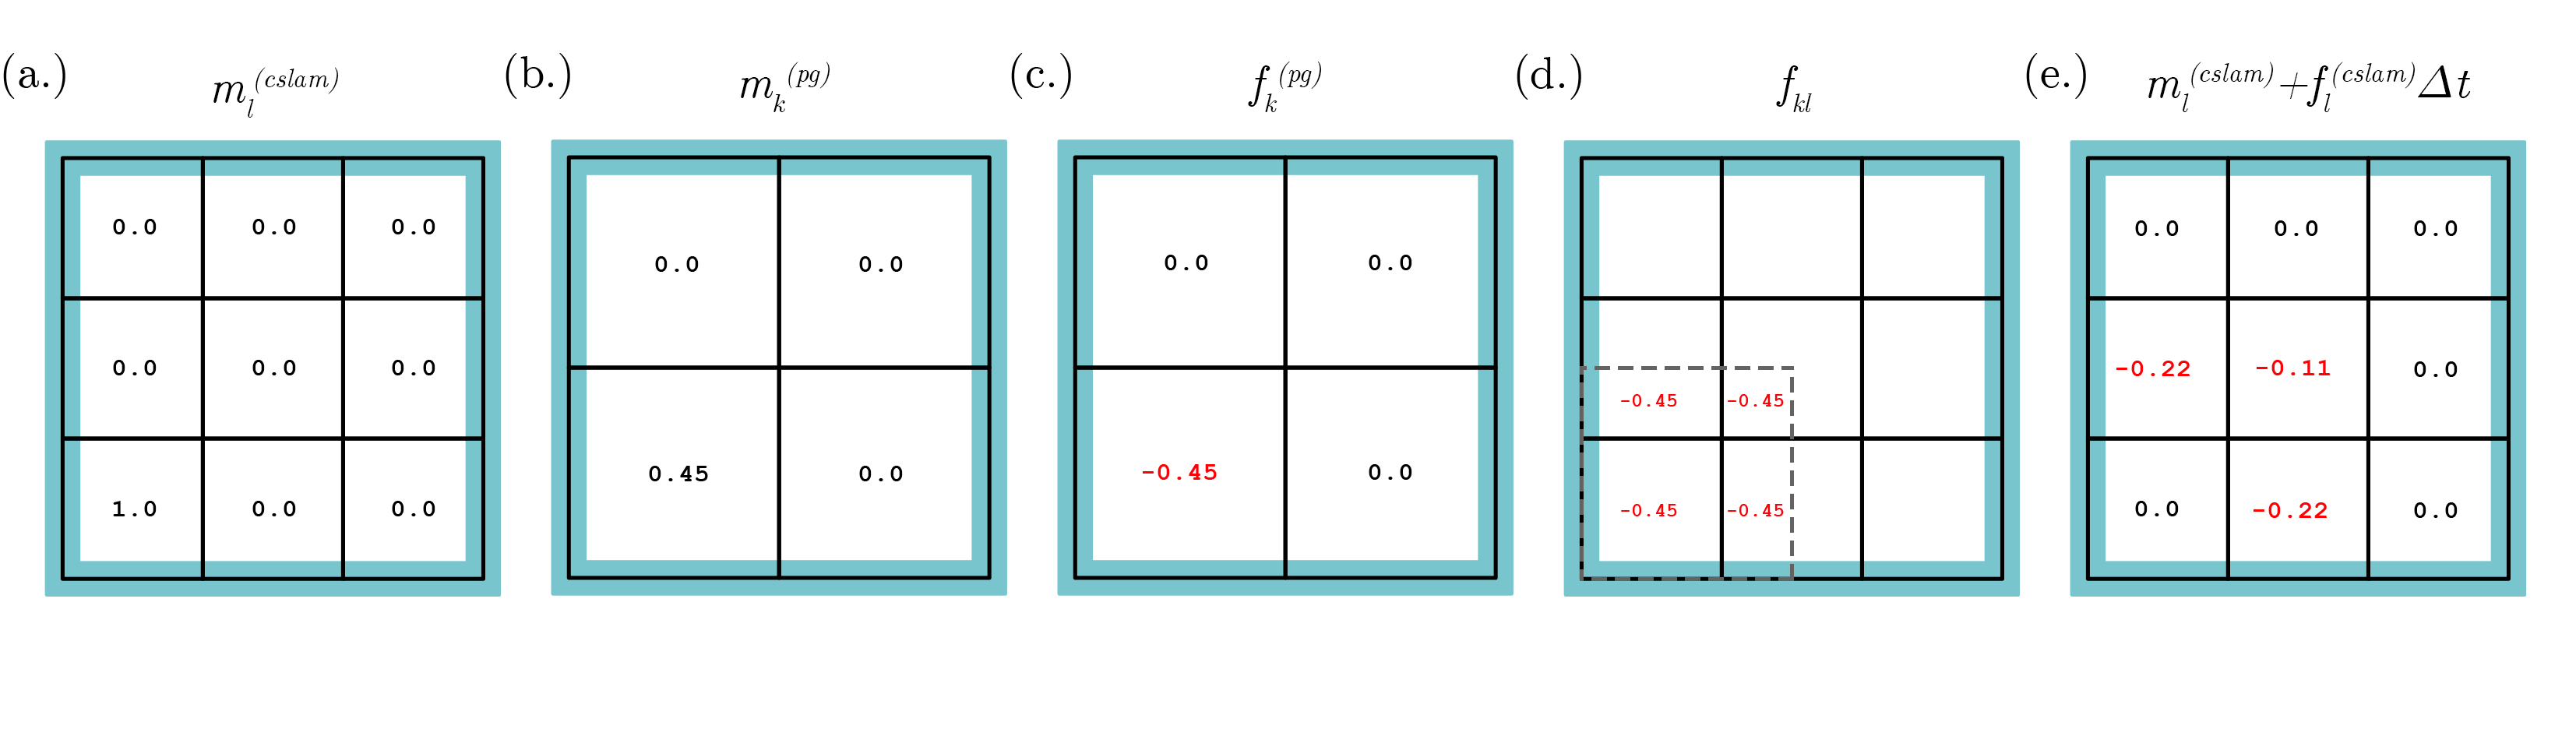
\includegraphics[width=30pc,angle=0]{figs/alg-schematic.png}\\
\end{center}
\caption{Schematic illustration of the `negativity problem' in a single element. (a.) Initial CSLAM tracer values, (b.) mapped to $pg2$, (c) produces a tracer increment on $pg2$, (d.) with negative increments on the exchange grid overlying CSLAM cells in (a) that were initially zero and (e) driving those mixing ratios negative.}
\label{fig:alg-schematic}
\end{figure}
\paragraph{The `negativity' problem and linear correlations} 
Even if one could derive a reversible map for mapping ${\overline{\Delta p}}^{(pg2)}$ from the physics grid to the CSLAM grid, there could still be problems if the increment drives the mixing ratios negative (or overshooting occurs) on the CSLAM grid. This can easily happen for tracers, such as cloud liquid amount and cloud ice amount, that are zero in most of the domain and non-zero in localized areas/points (where there are clouds). We refer to this as the `negativity problem'. This problem is depicted schematically in Figure~\ref{fig:alg-schematic}. Consider a single element of CSLAM control volumes, containing only a single cell with mixing ratio $1.0$, and $0.0$ everywhere else ($\overline{m}^{(pg3)}_\ell$; Figure ~\ref{fig:alg-schematic}a). The mixing ratios are mapped to the $pg2$ grid using, for simplicity, the piecewise constant method where a constant value inside the $pg2$ cells is used during the integration over overlap cells ($\overline{m}^{(pg2)}_k$; Figure~\ref{fig:alg-schematic}b). Now consider the case in which physics removes all the mass from the physics cell $k$: $\overline{f}^{(pg2)}_k=-\overline{m}^{(pg2)}_k$ (Figure~\ref{fig:alg-schematic}c). The tracer increment is mapped from $pg2$ to $pg3$ using the piecewise constant method. Some of the non-zero increments are now in overlap areas where the original CSLAM grid cells have mixing ratio zero ($\overline{f}_{k\ell}$; Figure~\ref{fig:alg-schematic}d), and hence, the state is driven negative when adding the overlap increment to the CSLAM state (Figure~\ref{fig:alg-schematic}e).  This is referred to as the negativity problem although it can also happen for maxima.

The negativity issue could be avoided if one remaps the physics updated state instead of mapping increments/tendencies. In that case a shape-preserving filter will make sure that the state on the CSLAM grid is not negative (and does not overshoot). That said, if physics does not change the state and it is mapped back to the CSLAM grid then spurious tendencies (proportional to the errors introduced by mapping state from the CSLAM grid to the physics grid and back again) are introduced. Hence it is advantageous to map increments/tendencies since any reasonable algorithm will preserve a zero function.

%In the $pg2$ configuration, mapping the fields to and from the quadrature grid and $pg2$ grid is identical to that described in H18. As discussed above above, in mapping to the physics grid, CAM-SE's Lagrange basis functions are integrated over the $pg2$ control volumes to provide the physics with a volume averaged state. The procedure is accurate to machine precision, conserves thermal energy and dry air mass, and is consistent (i.e., the mapping preserves a constant). The reverse mapping, from the physics grid to the quadrature grid, is done using a tensor-product Lagrange interpolation (see Appendix A in H18). The Lagrange interpolation is consistent, conserves dry air mass ({\color{red}{Peter, is this true?}}), but does not conserve thermal energy. Errors arising from the lack of energy conservation were estimated to be small; about two orders of magnitude less than the energy dissipation due to the dynamical core alone.

%The semi-Lagrangian advection of tracers in our $pg2$ configuration is solved on the CSLAM grid. 





%Interpolation: Traditional Lagrange interpolate of the mixing ratio increment would preserve a constant and could be made shape-preserving using {\em{ad hoc}} filters \citep[e.g.][]{BC2002MWR} but will not inherently preserve mass increment and suffers from the `negativity problem' described above.

As illustrated above a standard remapping method will NOT simultaneously satisfy 1-4 and hence a new algorithm has been derived.
\subsection{New tendency mapping algorithm}\label{sec:massfix}
Although this algorithm is explained and examined for a $pg2$ grid, it is general for any $pgX$ resolution. The problem is how to map the mass-increment on the physics grid, ${\overline{f}}^{(pg2)}\Delta A^{(pg2)}$, to the CSLAM cells that overlap with $\Delta A^{(pg2)}$. To maintain shape-preservation, linear correlations and to avoid the negativity problem locally, it is advantageous to define a mass excess function on the exchange grid $\Delta m_{k\ell}^{(excess)}$. It is basically the maximum amount of mixing ratio that can be removed (in the case ${\overline{f}}^{(pg2)}<0$) without producing new minima in the exchange grid mixing ratio $m_{k\ell}$
\begin{equation}
\Delta m^{(excess)}_{k\ell}=\overline{m}_{k\ell}-\overline{m}_k^{(min)},
\end{equation}
where $\overline{m}_{k\ell}$ is defined in \eqref{eq:moverlap2}. So the maximum amount of mass that we can be removed from the exchange grid cells that span physics grid cell $A_k$ without violating the shape-preservation constraint (\eqref{eq:min} and \eqref{eq:max}) is
\begin{equation}
\sum_\ell \Delta m^{(excess)}_{k\ell}\overline{\Delta p}_{k\ell} \delta A_{k\ell}.
\end{equation}
If physics is designed not to remove more mass than available in $A_k$ (which should be the case for a carefully designed physics package) then it is guaranteed that
\begin{equation}
\label{eq:well-posed}
\sum_\ell \Delta m^{(excess)}_{k\ell}\overline{\Delta p}_{k\ell} \delta A_{k\ell}\ge {\overline{f}}^{(pg2)}\Delta p_k\Delta A^{(pg2)}.
\end{equation}
We distribute the physics mass-forcing (assuming ${\overline{f}}^{(pg2)}<0$) according to the mass excess in each overlap area by solving this equation for $\gamma_k$
\begin{equation}
\label{eq:mass-excess}
\Delta A_k^{(pg2)}\overline{\Delta p}_k^{(pg2)}{\overline{f}}^{(pg2)}=\gamma_k \sum_\ell \Delta m^{(excess)}_{k\ell}\overline{\Delta p}_{k\ell} \delta A_{k\ell},
\end{equation}
and add mass increment (which in this case is negative)
\begin{equation}
\label{eq:mass-incr}
\gamma_k \Delta m^{(excess)}_{k\ell}\overline{\Delta p}_{k\ell} \delta A_{k\ell},
\end{equation}
to the $\ell$th CSLAM cell state ${\overline{m}}^{(pg3)} \overline{\Delta p}^{(pg3)}_\ell \Delta A^{(pg3)}_\ell$. This process is repeated for all physics cells. Note that this problem is a well-posed, i.e. $\gamma_k>0$, since physics will not remove more mass than is locally available \eqref{eq:well-posed}. The way in which the mass-forcing is distributed to the CSLAM cells using the excess function insures that the negativity problem is avoided. Mass is conserved by design and shape-preservation is obtained by using the excess function.

If the physics increment is positive (assuming ${\overline{f}}^{(pg2)}>0$) we define a `lack' function
\begin{equation}
\Delta m^{(lack)}_{k\ell}=\overline{m}_{k\ell}-\overline{m}^{(max)},
\end{equation}
and solve
\begin{equation}
\label{eq:mass-lack}
\overline{\Delta p}_k^{(pg2)}{\overline{f}}^{(pg2)}\Delta A_k^{(pg2)}=\gamma_k \sum_\ell \left[ \Delta m^{(lack)}_{k\ell}\overline{\Delta p}_{k\ell} \delta A_{k\ell}\right],
\end{equation}
for $\gamma_k$ and follow the same procedure as for mass excess. Since positive and negative forcing is treated in exactly the same way, linear correlations are preserved. Note how the definition of the excess/lack function insures linear correlation preservation; for example, if one would prevent negative values and not do anything about overshoots then linear correlations would not be preserved since the minima and maxima are not treated in the same way.

While the above algorithm satisfies properties 1-4 in section \ref{sec:pgtonc}, it is not a high-order algorithm in terms of formal accuracy. This is illustrated in Figure \ref{fig:mapping} (row 3) where a smooth analytical tendency \citep[approximate spherical harmonic of order 32 and azimuthal wave number 16; ][]{J1999MWR}
\begin{equation}
\label{eq:Y32}
f^{(pg2)}=\frac{1}{2}+\frac{1}{2}\cos(16\lambda)\sin(2\theta)^{16},
\end{equation}
where $(\lambda,\theta)$ is latitude-longitude, is mapped from $pg2$ to $pg3$ grid using this algorithm assuming $m^{(pg3)}_\ell=0, \quad \forall \ell$. The errors in the mapping are not always aligned with large gradients in the analytical function as would be expected for a `traditional' interpolation algorithm. The errors are maximum on the order of 60$\%$. To reduce errors we therefore perform a higher-order pre-allocation of tendencies that is not mass-conserving but satisfies properties 2,3, and 4 in Section \ref{sec:pgtonc}.

\begin{figure}[t]
\begin{center}
\noindent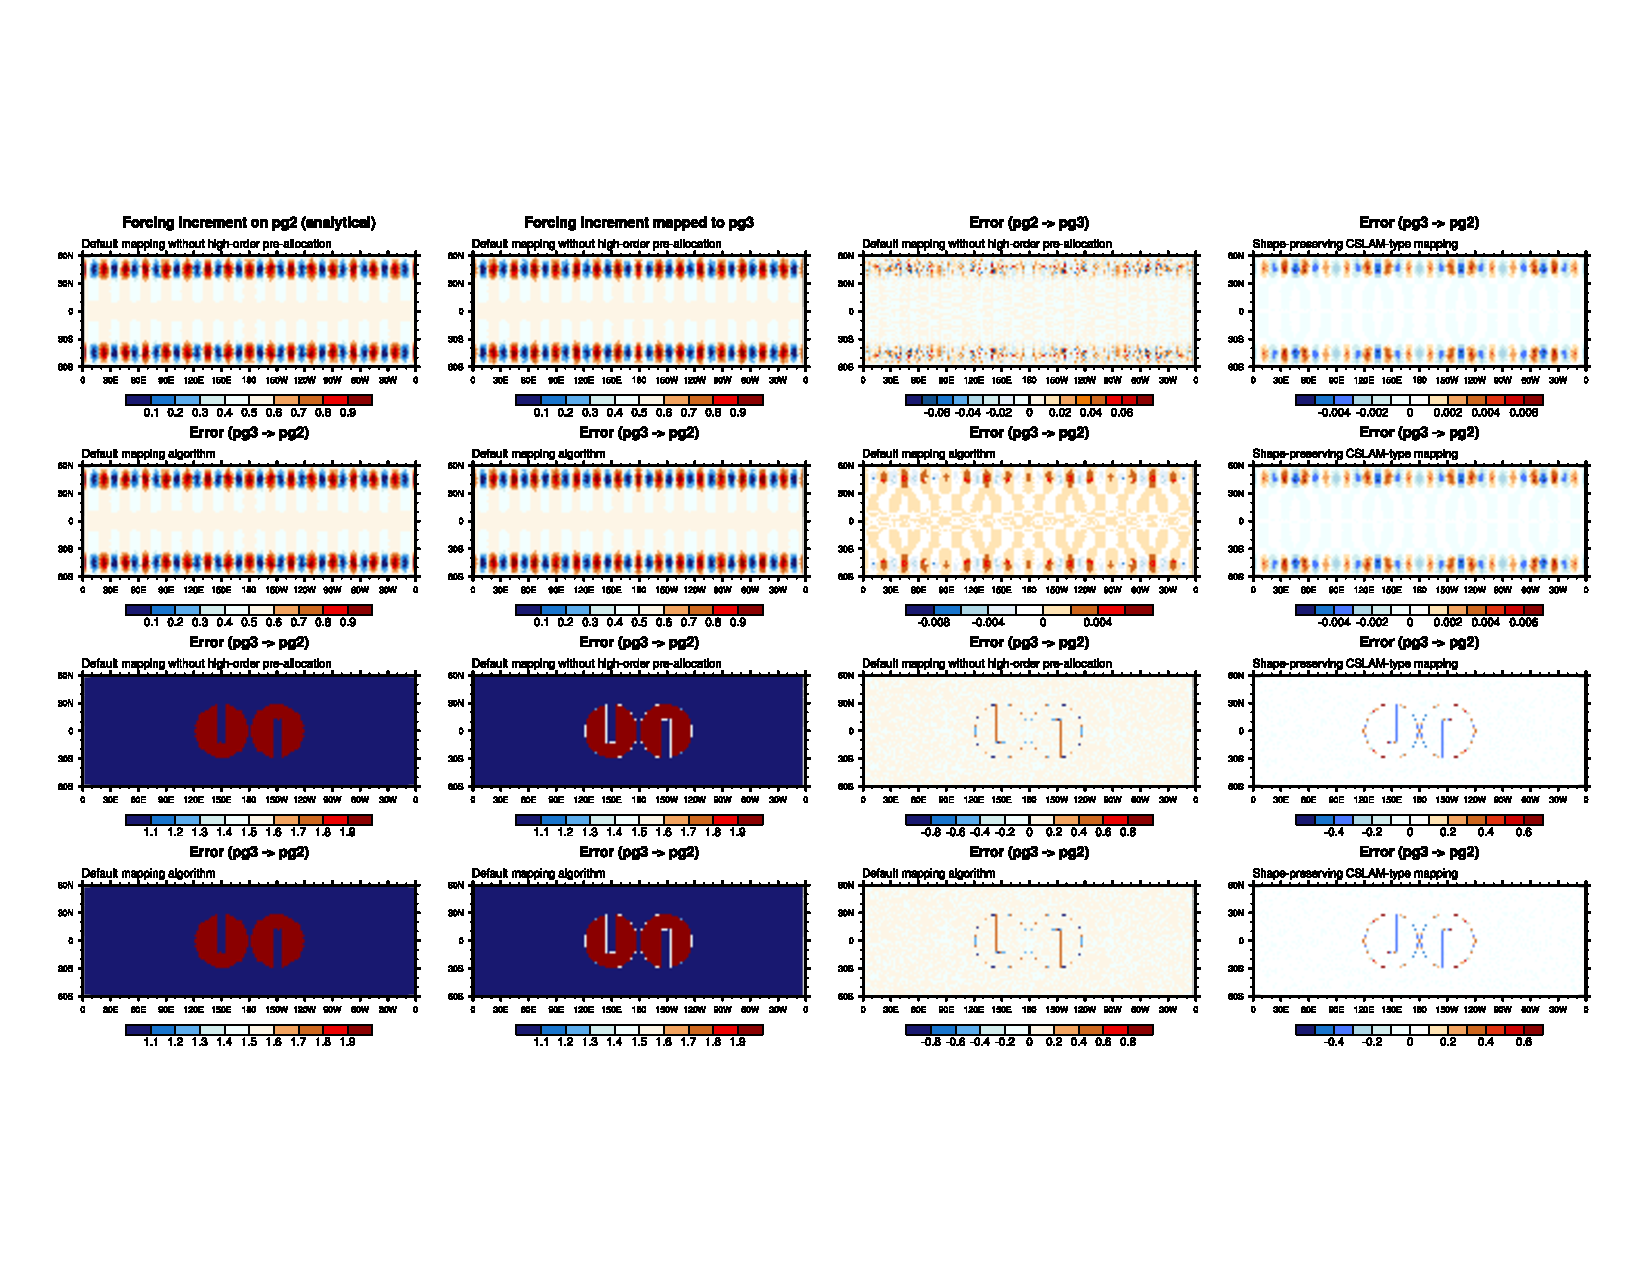
\includegraphics[width=30pc,angle=0]{figs/mapping.pdf}\\
\end{center}
\caption{Mapping of idealized functions from $pg2$ (column 1) to $pg3$ (columns 2) and errors (column 3) using the new tendency algorithm only (row 1 and 3) and new tendency algorithm with the high-order pre-allocation (row 2 and 4). Column 4 shows the errors in mapping the same distributions from  $pg3$ to $pg2$ using traditional remapping (CSLAM technology).}
\label{fig:mapping}
\end{figure}

%Similarly we define a mass lack function

%which is the maximum amount of mixing ratio that can be added without creating new maxima.

\subsection{High-order (non-conservative) pre-allocation of tracer tendencies}
A high-order tracer mass increment in overlap area $A_{k\ell}$ can be computed using the following formula
\begin{equation}
\label{eq:mp3}
\left< f\delta p\right>_{k\ell}=\int_{A_{k\ell}}\left[ \overline{\Delta p}_\ell^{(pg3)}\sum_{i+j\le 2}{\mathcal{F}}^{(ij)}_k x^{i}y^{j}+{\overline{f}}_k^{(pg2)}\sum_{i+j\le 2}{\widetilde{{\mathcal{P}}}}^{(ij)}_\ell x^{i}y^{j}\right] dA,
\end{equation}
where $\mathcal{F}^{(ij)}_k$ is the forcing increment reconstruction coefficients in the $k$th physics grid cell and ${\overline{f}}_k^{(pg2)}$ is the average physics increment in the $k$th physics grid cell. Note that we are using the known dry pressure reconstruction coefficients on the $pg3$ grid instead of reconstructing sub-grid-scale pressure variations from the physics grid cell averaged values. We can do that since the dry pressure is not modified by physics. This highlights the importance of a dry-pressure formulation of the dynamical core when separating physics and dynamics grids \citep{LetAl2018JAMES}. If the physics forcing is constant then $\left< f\delta p\right>_{k\ell}$ exactly equals $\left<\delta p\right>_{k\ell}$ from \eqref{eq:pg3dp}; in other words, the mapping is designed to be reversible in dry pressure. The physics increment in terms of mixing ratio change is given by
\begin{equation}
\label{eq:pg3fq}
\overline{f}_{k\ell}=\frac{\left< f\delta p\right>_{k\ell}}{\left<\delta p\right>_{k\ell}},
\end{equation}
where the denominator is given by \eqref{eq:pg3dp}.

Shape-preservation, as defined by \eqref{eq:min} and \eqref{eq:max}, is enforced by eliminating under and overshoots on the exchange grid by modifying the forcing increment $\overline{f}_{k\ell}$ so that shape-preservation is not violated in the overlap areas{\footnote{In the computation of $\overline{m}_{k\ell}$ there can be small overshoots and undershoots (due to numerical integration errors) compared to the CSLAM cell average values $\overline{m}^{(pg3)}_\ell$ that it overlaps with so we set
\begin{equation}
\overline{m}_k^{(min)}=\min \left( \overline{m}_k^{(min)},\left\{ \overline{m}^{(pg)}_\ell)|\ell=1,nc^2\right\} \right)
\end{equation}}}
\begin{equation}
\overline{m}_k^{(min)} \le \overline{m}_{k\ell}+\widetilde{\overline{f}}_{k\ell} \le \overline{m}_k^{(max)}.
\end{equation}
While this algorithm preserves linear correlations, shape, and is consistent, is it not mass-conservative. Hence the remaining physics increment not allocated in the algorithm above is allocated using the new tendency algorithm described in Section \ref{sec:massfix}.

Combining the high-order pre-allocation algorithm with the new tendency algorithm (which in this case can also be considered as a mass-fixer that does not disrupt correlation-preservation, shape and consistency) leads to an order-of-magnitude reduction in mapping errors for a smooth function (see Figure \ref{fig:mapping} row 3 and 4) while full-filling the mass-conservation, shape-preservation, linear correlation and consistency  constraint. Mass and linear correlation preservation is illustrated in the baroclinic wave test with terminator chemistry test in Section \ref{sec:fkessler}. Shape-preservation and consistency is demonstrated in an idealized mapping test where a smooth function, see \eqref{eq:Y32}, and a slotted-cylinder \citep[see equation 12 in ][]{LSPT2012GMD} are mapped to/from the $pg2$ and $pg3$ grids. Since the background value in the mapping of the slotted-cylinder field is preserved the mapping algorithm is consistent. Since no new over- and undershoots are produced (particularly obvious in the mapping of the slotted cylinders) the mapping is shape-preserving. We also note that the mapping errors with the default algorithm (higher-order pre-allocation with new tendency algorithm) are similar to the errors in mapping the same field from $pg3$ to $pg2$ using traditional remapping with CSLAM technology (column 4 in Figure \ref{fig:mapping}).


%A high-order estimate of the physics increment in the $A_{k\ell}$th overlap cell, that is not mass-conserving, can be computed as
%\begin{equation}
%\label{eq:mp3}
%\overline{f}_{k\ell}=\frac{1}{\delta A_{k\ell}}\int_{A_{k\ell}}\left[ \sum_{i+j\le 2}{\mathcal{F}}^{(ij)}_k x^{i}y^{j}\right] dA,
%\end{equation}
%where $\mathcal{F}^{(ij)}_k$ are the recontruction coefficients for the physics increment $f$ in the $k$th physics grid cell. For reasons that will become clear a shape-preserving limiter is not applied when computing $\mathcal{F}^{(ij)}_k$. Each overlap increment is added to the CSLAM opverlap state $\overline{m}_{k\ell}$ 
%\begin{equation}
%\overline{m}_{k\ell}+\tilde{\overline{f}}_{k\ell},
%\end{equation}
%where $\tilde{\overline{f}}_{k\ell}$ is $\overline{f}_{k\ell}$ `cropped' so that shape-preservation is not violated locally

% \section{Section title}
% \subsection{subsection one}
% text...
% \subsection{subsection two}
% \section{Section title}

%%%

\section{Results}

% \subsection{First secondary heading}

% \subsubsection{First tertiary heading}

% \paragraph{First quaternary heading}

%%%%%%%%%%%%%%%%%%%%%%%%%%%%%%%%%%%%%%%%%%%%%%%%%%%%%%%%%%%%%%%%%%%%%
% ACKNOWLEDGMENTS
%%%%%%%%%%%%%%%%%%%%%%%%%%%%%%%%%%%%%%%%%%%%%%%%%%%%%%%%%%%%%%%%%%%%%
%
\acknowledgments
NCAR is sponsored by the National Science Foundation (NSF).

%%%%%%%%%%%%%%%%%%%%%%%%%%%%%%%%%%%%%%%%%%%%%%%%%%%%%%%%%%%%%%%%%%%%%
% APPENDIXES
%%%%%%%%%%%%%%%%%%%%%%%%%%%%%%%%%%%%%%%%%%%%%%%%%%%%%%%%%%%%%%%%%%%%%
%
% Use \appendix if there is only one appendix.
%\appendix

% Use \appendix[A], \appendix}[B], if you have multiple appendixes.
%\appendix[A]

%% Appendix title is necessary! For appendix title:
%\appendixtitle{}

%%% Appendix section numbering (note, skip \section and begin with \subsection)
% \subsection{First primary heading}

% \subsubsection{First secondary heading}

% \paragraph{First tertiary heading}

%% Important!
%\appendcaption{<appendix letter and number>}{<caption>} 
%must be used for figures and tables in appendixes, e.g.,
%
%\begin{figure}
%\noindent\includegraphics[width=19pc,angle=0]{figure01.pdf}\\
%\appendcaption{A1}{Caption here.}
%\end{figure}
%
% All appendix figures/tables should be placed in order AFTER the main figures/tables, i.e., tables, appendix tables, figures, appendix figures.
%
%%%%%%%%%%%%%%%%%%%%%%%%%%%%%%%%%%%%%%%%%%%%%%%%%%%%%%%%%%%%%%%%%%%%%
% REFERENCES
%%%%%%%%%%%%%%%%%%%%%%%%%%%%%%%%%%%%%%%%%%%%%%%%%%%%%%%%%%%%%%%%%%%%%
% Make your BibTeX bibliography by using these commands:
\bibliographystyle{ametsoc2014}
\bibliography{bib}


%%%%%%%%%%%%%%%%%%%%%%%%%%%%%%%%%%%%%%%%%%%%%%%%%%%%%%%%%%%%%%%%%%%%%
% TABLES
%%%%%%%%%%%%%%%%%%%%%%%%%%%%%%%%%%%%%%%%%%%%%%%%%%%%%%%%%%%%%%%%%%%%%
%% Enter tables at the end of the document, before figures.
%%
%
%\begin{table}[t]
%\caption{This is a sample table caption and table layout.  Enter as many tables as
%  necessary at the end of your manuscript. Table from Lorenz (1963).}\label{t1}
%\begin{center}
%\begin{tabular}{ccccrrcrc}
%\hline\hline
%$N$ & $X$ & $Y$ & $Z$\\
%\hline
% 0000 & 0000 & 0010 & 0000 \\
% 0005 & 0004 & 0012 & 0000 \\
% 0010 & 0009 & 0020 & 0000 \\
% 0015 & 0016 & 0036 & 0002 \\
% 0020 & 0030 & 0066 & 0007 \\
% 0025 & 0054 & 0115 & 0024 \\
%\hline
%\end{tabular}
%\end{center}
%\end{table}

%%%%%%%%%%%%%%%%%%%%%%%%%%%%%%%%%%%%%%%%%%%%%%%%%%%%%%%%%%%%%%%%%%%%%
% FIGURES
%%%%%%%%%%%%%%%%%%%%%%%%%%%%%%%%%%%%%%%%%%%%%%%%%%%%%%%%%%%%%%%%%%%%%
%% Enter figures at the end of the document, after tables.
%%
%
%\begin{figure}[t]
%  \noindent\includegraphics[width=19pc,angle=0]{figure01.pdf}\\
%  \caption{Enter the caption for your figure here.  Repeat as
%  necessary for each of your figures. Figure from \protect\cite{Knutti2008}.}\label{f1}
%\end{figure}

\end{document}
